

\afterpage{\null\newpage}
\chapter{Adaptive Sampling Comparison\label{ch:chapter32}}

One major challenge in developing, investigating and comparing adaptive sampling strategies is the large computational resources required to run adaptive sampling with the necessary molecular dynamics trajectories. To reach statistically significant sample sizes requires even larger computational resources rarely available.
The alternative of investigating adaptive sampling for toy systems or small peptides requires lower amount of computational resources. The lower dimensionality of these smaller test systems reduces the transferability of the resulting conclusions to biomoleculer which have order of magnitude more degrees of freedom and a more complex energy landscape. Some strategies which work well for toy systems of small peptides have significant challenges to scale up to larger proteins. One answer to this challenge in accurately investigating adaptive sampling strategies is the utilization of Markov Chain trajectories. These approximations of molecular dynamics trajectories can be generated many orders of magnitudes faster than molecular dynamics trajectories when the Markov State Model of a protein is known. Toy systems have 

The material in this chapter was first published in: 

\cite{Adstrategies2018} \textbf{Hruska, E.}; Abella, J. R.; N\"uske, F.;
Kavraki, L. E.; Clementi, C.; Quantitative
comparison of adaptive sampling methods
for protein dynamics. J. Chem. Phys.
2018, 149 


X
In order to be able to benchmark and compare the results on different systems, we
use previously generated extensive MD trajectories \cite{lindorff2011} to
generate 8 discrete models for protein dynamics.
The results of this analysis reveal that different strategies are needed
for different goals. In particular, on-the-fly estimation of global
equilibrium properties from non-equilibrium data is very important to speedup
the folding of a protein, while the knowledge of equilibrium properties is not
needed if the goal is the exploration of large regions of the conformational
space (independently if folded or unfolded). This result suggests that
different strategies may need to
be combined in various stages of a specific application to both enhance the
occurrence of a rare event and appropriately sample the different metastable states.
Comparison of the results on different proteins
suggest that the speedup that can be achieved by adaptive sampling is larger
for slower processes, thus encouraging the application to more complex systems.



\section{\label{sec:methods}Methods}


\subsection{\label{sec:methods-dataset}Reference Dataset of Simulations}

We used previously existing long all-atom MD trajectories
of 8 different small proteins\cite{lindorff2011}, obtained on the Anton supercomputer, to generate
discrete model systems, as discussed below. The dataset is summarized in Table
\ref{tab:dataset-summary} and contains proteins ranging from 10 to 80 residues,
with different topologies ($\alpha$-helices, $\beta$ sheets, or a mix of both),
simulated folding times ranging from $0.6$ to $49$ $\mu$s, and different timescale gaps between
the folding process and other competing slow processes.

\begin{table}[!ht]
\centering
\caption{Previously simulated proteins used to generate discrete models in this study}
\label{tab:dataset-summary}
%\begin{tabular}{ccccc}
\resizebox{\columnwidth}{!}{
\begin{tabular}{|c|c|c|c|c|c|}
\hline
Protein Name & PDB ID of Folded Structure & Size (\# residues) & Folding Time ($\mu$s) from \cite{lindorff2011}\\ 
\hline
Chignolin    & 2RVD                       & 10                 & 0.6                 \\
Trp-cage     & 2JOF                       & 20                 & 14                  \\
BBA          & 1FME                       & 28                 & 18                  \\
WW Domain    & 2F21                       & 35                 & 21                 \\
Protein B    & 1PRB                       & 47                 & 3.9                  \\
Homeodomain  & 2P6J                       & 52                 & 3.1                  \\
$\alpha$3D   & 2A3D                       & 73                 & 27                  \\
$\lambda$-repressor  & 1LMB               & 80                 & 49             \\ 
\hline            
\end{tabular}
}
\end{table}

\subsection{\label{sec:methods-msm}Construction of discrete protein models}

To emulated adaptive sampling, an MSM was generated for each protein from
the previously existing long all-atom MD trajectories, then synthetic
microstate trajectories are generated by sampling the MSM transition matrix.
An MSM models the system's dynamics by discretizing the explored
conformational space into a finite number of states, and estimating their
probability and the probability of transition between them \cite{prinz2011markov}.
The analysis is summarized by a transition matrix,
$T_{ij}$, that indicates the probability that the system transitions from state
$i$ to state $j$ within a chosen lag time $\tau$. The discretization of the
original conformational space into states (also called microstates) is usually
performed by clustering the configurations sampled by MD trajectories using
a distance metric that can separate slowly mixing configurations from rapidly
interconverting ones \cite{noe2016commute, Noe2015}.

We have used standard procedures to perform these steps. In particular, for
each protein, we used the Time-lagged Independent Component Analysis (TICA) 
\cite{TICA1-perez2013, TICA2-schwantes2013} combined with the commute map 
\cite{noe2016commute}, to reduce the dimensionality of the system. As an input
for TICA, each conformation was first featurized using all pairwise
inter-residue distances (between the two closest heavy-atoms) and all dihedral
angles along the protein chain.
For smaller systems, the reciprocals of the inter-residue distances were also
used as additional features. The Euclidean distance between the
lower-dimensional points in the commute map space provides a good measure to
obtain a kinetically meaningful state decomposition, and an associated MSM
\cite{noe2016commute}. All conformations were then
partitioned with k-means clustering into 1000 or 2000 microstates, depending on
the size of the protein. It was ensured that the slowest MSM eigenvector is the
folding-unfolding process and all microstates are connected by removing
disconnected microstates. Finally, the transition matrix for the MSM is
computed using maximum-likelihood estimation with a detailed balance
constraint. The lag time, $\tau$, for the MSM was chosen based on the
convergence of the implied timescales, and the Markovianity property of the MSM
was tested by using the Chapman-Kolmogorov test \cite{prinz2011markov}. All the
analysis was performed using the PyEMMA Python package \cite{scherer2015pyemma}
and the exact parameters for the construction of discrete protein models for
each protein are listed in the Supplementary material.

X create markov Chain trajectories

\subsection{\label{sec:level5}Simulating adaptive sampling with Markov Chain trajectories}
\RED{recerence chapter 3 Figure~\ref{fig:schema2}  }
Adaptive sampling involves iteratively running many short MD trajectories, and
different adaptive sampling methods differ in how the new structures are chosen
to initialize the next round of MD trajectories. We can simulate the adaptive
sampling process of iteratively running an ensemble of $n$ MD trajectories 
using the transition matrix from an MSM as follows. 
Note that the restart strategies here are concerned with selecting states
visited among the discrete set of microstates in the MSM. 
In actual molecular dynamics simulations, continuous trajectories in a protein
configurational space are used instead of the synthetic trajectories generated here
by jumping between the different discrete states of an MSM in adaptive step 2.
Therefore, in actual simulations the analysis (adaptive step 3 below) involves also the
the discretization of all the available trajectories into a set of microstates.


We denote the adaptive steps 3 and 4 together as the \emph{restart strategy} for an
adaptive sampling method. Figure~\ref{fig:schema} is a graphical representation
of the process. The different restart strategies that we use in this work are
described in detail in the following section. When using continuous trajectories from actual molecular dynamics simulations,
the analysis step 3 also includes the discretization of the continuous
trajectories into discrete trajectories (for instance, by means of TICA and MSM).
Thus, the restart strategy for adaptive sampling in actual molecular dynamics
simulations must also select a set of individual conformations or frames from the selected
microstates to initialize the next MD simulation. This can be done for example in
a uniformly random fashion within the microstate or by selecting a representative
conformation. 
The length of the trajectories in each iteration can be varied, but it needs to
be larger than the lag time used to generate the MSM.
Here we chose the length of each short MD trajectory the same as the lag time
$\tau$, that is, the analysis is performed after the discrete trajectories have
been propagated by one step of length $\tau$. 
At each iteration, for a given strategy, the $n$ restarting points for the new
trajectories are chosen independently of each other.

In order to study the speedup in folding, subsets of the discrete microstates for
each protein are denoted as folded and unfolded states. 
Using the PDB files from Table \ref{tab:dataset-summary}, the native contacts
are extracted for the folded structure of each protein. A native contact is
defined if the distance between the two closest heavy atoms in a pair of
residues is 4\r{A} or less. For each state in the MSM, we compute the median number of native
contacts over all the conformations mapped to the state. States above a threshold
value for the number of native contacts are assigned as a folded state. States
below a threshold value for the number of native contacts are assigned as an
unfolded state. The threshold values for individual proteins can be found in the Supplementary material. 




\section{\label{sec:results}Results}

In order to quantify the performance of different adaptive sampling strategies,
we considered two broad measures of efficiency. The first measure is the time
it takes for a strategy to simulate a rare event, in terms of steps of synthetic
trajectories. For the dataset used here, the rare event of interest is the
folding process and, for all proteins considered, the slowest timescale (or
rarest event) is the folding timescale. For each strategy, the average time measured
for a given strategy to reach the folded state starting from an unfolded state
is compared with the corresponding time in the absence of adaptive sampling
(that is, for the MD strategy described above). The second measure is one
that focuses on the exploration of the configurational space instead of a single
rare event. For any given strategy, we measure the time needed to explore 95\%
of the states used to build the MSM and compare it with the corresponding MD time.
For each protein, we evaluate these two measures for each of the adaptive
sampling strategies described above. Each strategy is evaluated by using a different
number of parallel trajectories $n$, ranging from 1 to 5000. 
The results reported
are averaged over 100 independent runs per protein and per number of parallel
trajectories.

\subsection{\label{sec:time-fold}Time to fold}

\begin{figure}[H]
  %%\centering
  \begin{subfigure}[t]{0.5\textwidth}
    \includegraphics[width=0.9\textwidth]{figures/CLN025_7_steps10000_nparallel100_fold.eps}
    %%\caption{Chignolin}    
  \end{subfigure}
  \begin{subfigure}[t]{0.5\textwidth}
    \includegraphics[width=0.9\textwidth]{figures/GTT_7_steps10000_nparallel100_fold.eps}
    %%\caption{WW Domain}    
  \end{subfigure}
  \begin{subfigure}[t]{0.5\textwidth}
    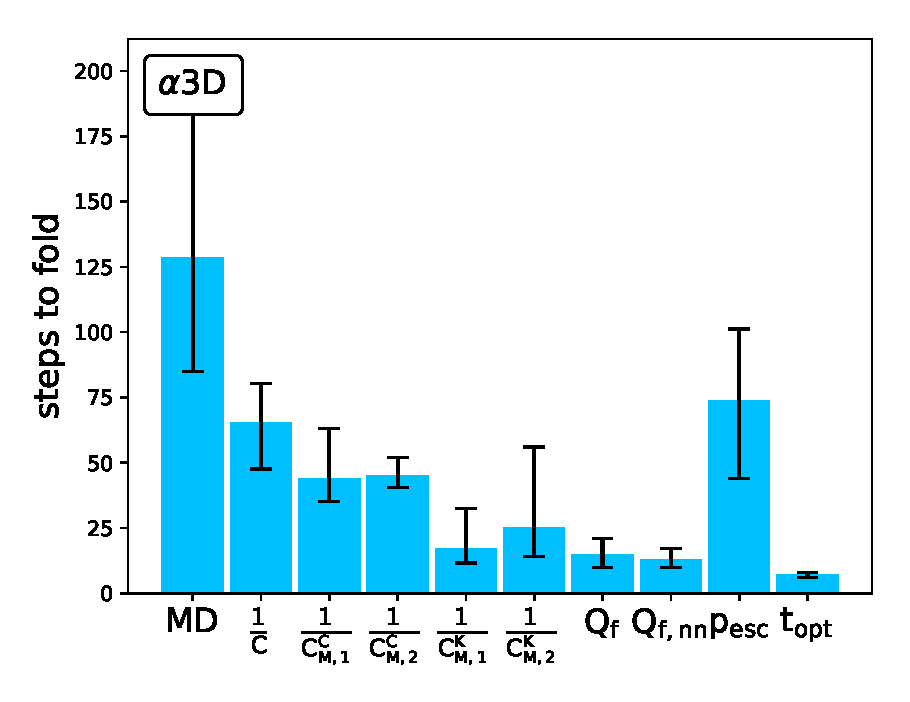
\includegraphics[width=0.9\textwidth]{figures/A3D_7_steps10000_nparallel100_fold.eps}
    %%\caption{$\lambda$-repressor}    
  \end{subfigure}
  \caption{Comparison of the number of steps of synthetic trajectories required
  to fold for the different adaptive sampling strategies for three different
  proteins using 100 parallel trajectories. The 20\% and 80\% percentiles are
  shown as the error bars. The results of the t-test between MD and the
  individual strategies for the different proteins are reported in the Supplementary material.}
  \label{fig:Time_fold}
\end{figure}

Figure~\ref{fig:Time_fold} shows the average folding time for each of the
strategies for three different proteins using 100 parallel trajectories. First, we note that the
popular microstate-based $1/C$ strategy does not always appear to speedup the
folding time, while the macrostate-based methods do show significant
improvement over MD. 
Interestingly, the benchmark strategy designed to maximize the probability to
visit unexplored regions of the configurational space  ($p_{esc}$, defined
above) does not significantly speedup the sampling of the folding rare event.
Both $1/C$ and $p_{esc}$ are strategies designed for general exploration and
not specifically for rare event sampling, and it is not surprising that these
strategies do not perform well in accelerating folding events.
Instead, the macrostate-based methods appear to successfully introduce a
sampling bias toward states that are along the direction of the slowest
timescale, as manifested in the significant speedup with respect to simple MD.
These results are consistent over the set of model proteins studied.

Within the macrostate-based methods, the correction for non-equilibrium that
can be achieved by Koopman reweighting ($1/C_M^K$) appears to further improve
the sampling of the rare folding event over using a simple uncorrected count
matrix ($1/C_M^C$) in the on-the-fly MSM definition. The correction for
non-equilibrium allows a more accurate estimation of the leading eigenvector of
the true transition matrix over using the raw, on-the-fly count matrix. Thus,
the resulting macrostates are more kinetically relevant. We also observe that
the results obtained when the number of macrostates is defined by the kinetic
content ($1/C_{M, 2}$) do not differ significantly from what is obtained when a constant number
of macrostates is used ($1/C_{M, 1}$). In some instances, it appears that using
kinetic content slightly hurts the performance of the adaptive sampling, which
may be due to inaccurate estimation of the timescales in the early stages
of the simulation.

Finally, we observe that incorporating a reaction coordinate, such as the
number of native contacts in the strategies does indeed significantly improve
the sampling of rare events. The improvement is, in fact, close to the
theoretical maximum that is estimated by $t_{opt}$. We also observe that the
addition of the number of non-native contacts as a second reaction coordinate
does not always improve the performance of the algorithm. In particular, this
is true for the smallest of the protein model considered (Chignolin), the
kinetics of which does not exhibit any additional slow processes besides
folding (see Fig.~\ref{fig:Time_fold}). For all the other protein models, the
introduction of a second reaction coordinate very marginally improves the
sampling of the folding process.
These patterns are consistent across all the proteins and across the number of
parallel trajectories used. The plots for all proteins (in addition to
Fig.~\ref{fig:Time_fold}) can be found in the Supplementary material.


\subsection{\label{sec:time-explore}Time to explore 95\% of states}

\begin{figure}[H]
  %%\centering
  \begin{subfigure}[t]{0.5\textwidth}
    \includegraphics[width=0.9\textwidth]{figures/CLN025_7_steps10000_nparallel100_explore.eps}
    %%\caption{Chignolin}   
    %%[width=\textwidth] 
  \end{subfigure}
  \begin{subfigure}[t]{0.5\textwidth}
    \includegraphics[width=0.9\textwidth]{figures/1FME_7_steps10000_nparallel100_explore.eps}
    %%\caption{WW Domain}    
  \end{subfigure}
  \begin{subfigure}[t]{0.5\textwidth}
    \includegraphics[width=0.9\textwidth]{figures/A3D_7_steps10000_nparallel100_explore.eps}
    %%\caption{$\lambda$-repressor}    
  \end{subfigure}
  %%\includegraphics[width=\textwidth]{figures/UVF_7_steps10000_nparallel100_explore.eps}
  \caption{Comparison of the number of steps required to explore 95\% of the
  configurational space for different adaptive sampling strategies for three
  different protein models, by using 100 parallel trajectories. The 20\% and
  80\% percentiles are shown as the error bars.
  The results of the t-test between MD and the
  individual strategies for the different proteins are reported in the Supplementary material.}
  \label{fig:Time_explore}
\end{figure}

Figure~\ref{fig:Time_explore} shows the average time needed for the different
adaptive sampling strategies to explore 95\% of the microstates constituting the
MSM, by using 100 parallel trajectories, for three different proteins.
In this comparison we exclude the strategies designed to speedup the sampling
of the folding process (such as the native contact based strategies as well as
$t_{opt}$) because they are not designed for the purpose of general exploration.
The comparison shows that, in general, the $1/C$ strategy explores the
configurational space much more efficiently than plain MD. The speedup obtained
by the $1/C$ strategy nears the theoretical maximum obtained by the optimal
exploration strategy, $p_{esc}$. Within the macrostate-based strategies, there
is more variance. The strategies using the regular count matrix $(1/C_M^C)$ outperform
the strategies that correct for non-equilibrium errors, $(1/C_M^K)$. This is
likely because the correction introduces a bias towards the sampling of slow
processes rather than general exploration. The non-equilibrium error in the
count matrix based strategies introduces randomness that helps the sampling of
unexplored microstates. Additionally, for some proteins the optimization of the number of
macrostates based on the kinetic content ($1/C_{M, 2}$) does appear to provide
an advantage over the use of a constant number of macrostates ($1/C_{M, 1}$). 
The use of the kinetic content allows for a more accurate estimation of
macrostate counts, which could help to focus the sampling bias towards regions
that are less densely sampled. 
The patterns shown in Fig.~\ref{fig:Time_explore}
are consistent across all the proteins and across the number of
parallel trajectories used. The corresponding plots for all the proteins can be
found in the Supplementary material.

\subsection{\label{sec:scaling}Scaling}

\begin{figure}[H]
  %%\centering
  \begin{subfigure}[t]{0.5\textwidth}
    \includegraphics[width=0.9\textwidth]{figures/GTT_6_steps10000_scaling_fold0.eps}    
  \end{subfigure}
  \begin{subfigure}[t]{0.5\textwidth}
    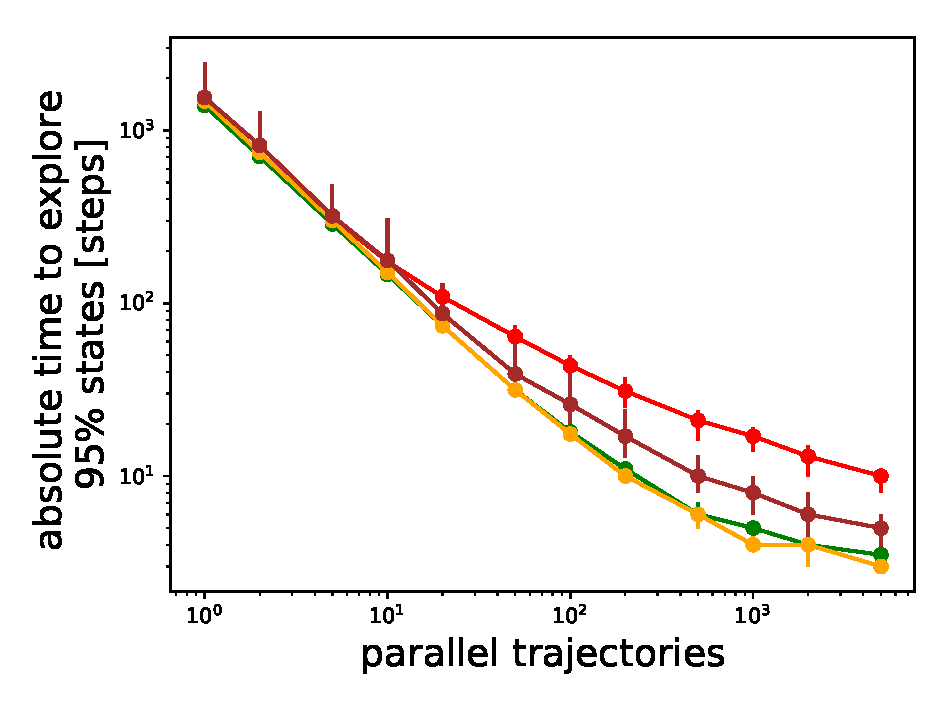
\includegraphics[width=0.9\textwidth]{figures/1FME_6_steps10000_scaling_explore.eps}
    %%\caption{$\lambda$-repressor}    
  \end{subfigure}
  \begin{subfigure}[t]{0.5\textwidth}
    \includegraphics[width=0.9\textwidth]{figures/1FME_6_steps10000_scaling_explore_total.eps}
    %%\caption{$\lambda$-repressor}    
  \end{subfigure}
  \caption{Top: Scaling of the absolute folding time required to fold the
  protein model for the WW Domain for 5 different sampling strategies: plain
  $MD$, $p_{esc}$, $t_{opt}$, $1/C$ and $1/C_{M,2}^K$. Scaling of the
  absolute (middle) or cumulative (bottom) number of steps required to explore
  95\% of all microstates, for the protein  model of BBA, for 3 different
  strategies: plain $MD$, $p_{esc}$, $1/C$ and $1/C_{M,2}^K$.  
  The 20\% and 80\% percentiles are shown as error bars. 
  Similar figures for the other
  protein models are reported in the Supplementary material.}
  \label{fig:scaling}
\end{figure}

Adaptive sampling methods capitalize on the use of many relatively short
parallel trajectories, usually deployed on massively parallel computers (MPC),
to speed up rare events or explore protein conformational spaces. In order to
better understand the limits of scalability of adaptive sampling strategies,
the measured absolute folding time for different parallelization is shown in
Figure \ref{fig:scaling}. The absolute folding time indicates the actual clock
time required to record a folding event for a given protein on MPC with a given
adaptive sampling strategy. The different strategies exhibit good scaling below
a parallelization of around 100 and moderate scalability up to 1000 parallel
trajectories. The scalability differs only slightly between different
strategies, confirming that adaptive sampling generally scales well.
Similar scaling is observed for all protein models. The time to explore 95\% of
microstates in Figure \ref{fig:scaling} scales to a higher parallelization than
the time to fold the protein. In addition to Fig.
\ref{fig:scaling}, scaling plots for the other protein models are
available in the Supplementary material. 

\begin{figure}[H]
  %%\centering
  \begin{subfigure}[t]{0.5\textwidth}
    \includegraphics[width=0.9\textwidth]{figures/compare_MD_speed_up_t_opt_6_steps10000_52_0.eps}
    %%\caption{$t_{opt}$}    
  \end{subfigure}
  \begin{subfigure}[t]{0.5\textwidth}
    \includegraphics[width=0.9\textwidth]{figures/compare_MD_speed_up_qcore_only_6_steps10000_52.eps}
    %%\caption{$Q_f$}    
  \end{subfigure}
  \begin{subfigure}[t]{0.5\textwidth}
    \includegraphics[width=0.9\textwidth]{figures/compare_MD_speed_up_cmacro_kin_cont_50_6_steps10000_52.eps}
    %%\caption{$1/C_{M,2}^K$}
  \end{subfigure}
  \caption{The relationship between the speedup of the folding time with $t_{opt}$, $Q_f$
  or $1/C_{M,2}^K$ vs. mean first passage time for the 8 proteins. Results are reported for a
  parallelization of 100, and the 20\% and 80\% percentiles are shown as error
  bars. The speedup increases with longer MD folding time, the linear fit lines are drawn to guide the eye. The Pearson
  correlation coefficient is for $t_{opt}$ 0.93, for $Q_f$ 0.95 and for
  $1/C_{M,2}^K$ 0.82.}
  \label{fig:compare-MD-speed-cmacro}
\end{figure}


\subsection{\label{sec:compare}Speedup for different proteins}

The speedup in simulating the folding process achieved by using adaptive
sampling in Figure~\ref{fig:Time_fold} varies for different proteins as each
protein has different dynamic properties. In order to better understand the
factors determining the speedup reachable with adaptive sampling strategies, we
compare different properties over the different protein models.

Figure \ref{fig:compare-MD-speed-cmacro} shows that, despite the small sample size
and large error bars, there is a significant correlation between
the theoretical maximum speedup in folding reachable with adaptive sampling
($t_{opt}$) and the folding time of a protein model (as measured by the mean first passage time).
Similar correlations appear for the speedup achieved by using an adaptive
sampling strategy based on the number of macrostates explored upon correction
for non-equilibrium effect ($1/C_{M, 2}$), and also when a reaction coordinate
is used to guide the adaptive sampling ($Q_f$).
That is, for slower folding proteins the efficiency of adaptive sampling
strategies in accelerating the folding rare event increases. This result is
very encouraging for the use of adaptive sampling strategies to sample slow
processes, as adaptive sampling seems to perform better as the processes become
slower. The large error bars are caused by the stochastic nature of the
trajectories. 
No significant correlation is observed between the speedup achieved in folding
and additional properties such as the size of the protein (Figures in Supplementary material).


\section{\label{sec:conclusion}Conclusion}

We have presented a systematic analysis of the performance of different
adaptive sampling strategies by using as test systems 8 different discrete
protein models defined from long all-atom MD simulations.
We have shown that different adaptive sampling strategies are optimal for
different goals. In particular, if the goal of adaptive sampling is to speedup
the simulation of a rare event (such as a protein folding process), it is
important to be able to analyze the explored space on-the-fly and extract a few
metastable states from which new simulations can be restarted. In the data
analysis, it is also important to take into account the effect of
non-equilibrium sampling. Indeed, our results show that a more accurate
estimation of an equilibrium MSM from short non-equilibrium simulations, that
can be obtained by using corrections based on the estimation of the Koopman
operator \cite{koopmanold, koopman2,koopman3,koopman4,  wu2017variational,
Nueske2017}, significantly improve the adaptive sampling of a
protein folding process with respect to a simple estimation of the MSM directly
from non-equilibrium transition counts.

Different considerations are important if the goal of adaptive sampling is to
speedup the exploration of any new regions of the configurational space of a
protein system. In this case, it appears that the most efficient adaptive
sampling strategy is based on the on-the-fly identification of a large number
of kinetic microstates from the simulations already performed, and corrections
for non-equilibrium effects do not appear relevant.
These results suggest that different strategies could be used in different
stages of investigation of a given biophysical process. For instance, the
sampling of rare events could be optimized in a first stage to discover slow
processes in a new system of interest, followed by a second stage where the
different metastable regions in the conformational space can be better sampled
by an adaptive sampling strategy optimized for fast exploration.

We have compared the speedup achieved with the different adaptive sampling
strategies with theoretically optimal benchmark strategies for these two
different goals, $p_{esc}$ and $t_{opt}$, respectively.  The gap between the
speedup of the theoretically optimal strategies and the best performers among
the strategies presented suggest that there could be even faster 
adaptive sampling methods and further investigation in this direction is underway.

We have also shown that, if there is a priori knowledge about the process
under investigation, as for example a reaction coordinate, then adaptive
sampling strategies for the sampling of rare events can be designed to achieve
a speedup close to the theoretical maximum benchmark. In particular, we have
shown that using the number of native (and non-native) contacts to guide the sampling, a
significant improvement in the adaptive sampling of the folding process is
obtained with respect to adaptive sampling strategies that do not use a priori
knowledge of the system.

The adaptive sampling strategies reported here scale well with parallelization
up to about 1000 for the investigated systems.  This result generalizes what
was reported in \cite{bowman2010enhanced} for different proteins. 

Although the best performing adaptive sampling strategies presented here show a
robust speedup over plain MD over a number of different protein models, a significant
variation in performance is observed. Interestingly, the
speedup obtained with the best performing adaptive sampling strategies for
the sampling of the folding process for different protein models correlates
with the folding time as measured with plain MD simulations.
Instead, the size of the proteins or the height of the folding free energy
barrier for the different proteins do not appear to be a strong determinant for
the speedup obtainable by adaptive sampling.
A cautious extrapolation of the correlation between the adaptive sampling
performance and the timescale of the folding rare event encourages the
application of these methods for the characterization of slower processes,
beyond the fast-folding proteins considered here. Due to the limited
number of investigated proteins and the discrete nature of the models used,
the upper limit of the speedup achievable with adaptive sampling methods
for the sampling of rare events cannot be directly estimated from what is
presented here.



X Discuus approcimation markov chain trajetcorie to molecular dynamics trajctories 